% È roba un po' confusa, è prima mattina per tutti. Se hai capito meglio quello
%che il prof voleva dire sei libero di mettere a posto :D
Un attaccante può tentare di modificare il messaggio ma quello che gli mancherà
sarà $k$, ovvero la mia chiave con cui cifro il messaggio.
L'attaccante allora potrebbe provare a sostituire la chiave $k$, e il difensore
non si accorgerebbe di nulla. Questo metodo funziona quando il file ha quindi
una struttura, ed è presente un'alta entropia.

Non si firma mai il messaggio perché è molto oneroso ($m^d$ con $m$ molto
grande), quello che si fa è applicare l'hash al messaggio e fare la firma
dell'hash del messaggio.

$$
m \rightarrow h(m) \rightarrow s(h(m))
$$

La firma è

$$
\langle m, h(m), n \rangle
$$

Per verificare prendo il messaggio, calcolo l'hash e lo confronto con l'hash
ricevuto del messaggio. Se sono uguali la comunicazione è andata a buon fine.
Questo garantisce l'autenticità del messaggio e il non ripudio.

Il non ripudio è qualcosa di fondamentale per permettere il commercio. Il non
ripudio è possibile perché si è in grado di \textbf{firmare}. La firma digitale
implementa il non ripudio nel mondo elettronico.

\paragraph{Public Key Infrastructure}

Una \textit{Certification Authority} è una struttura che gestisce la
\textit{catena di trust}. In Italia sono presenti queste società che permettono
di firmare in maniera digitale documenti, con valore legale. Questo avviene
perché quando si va ad aprire un account è necessario presentare a mano la
propria carta d'identità.


\begin{figure}[H]
 \centering
 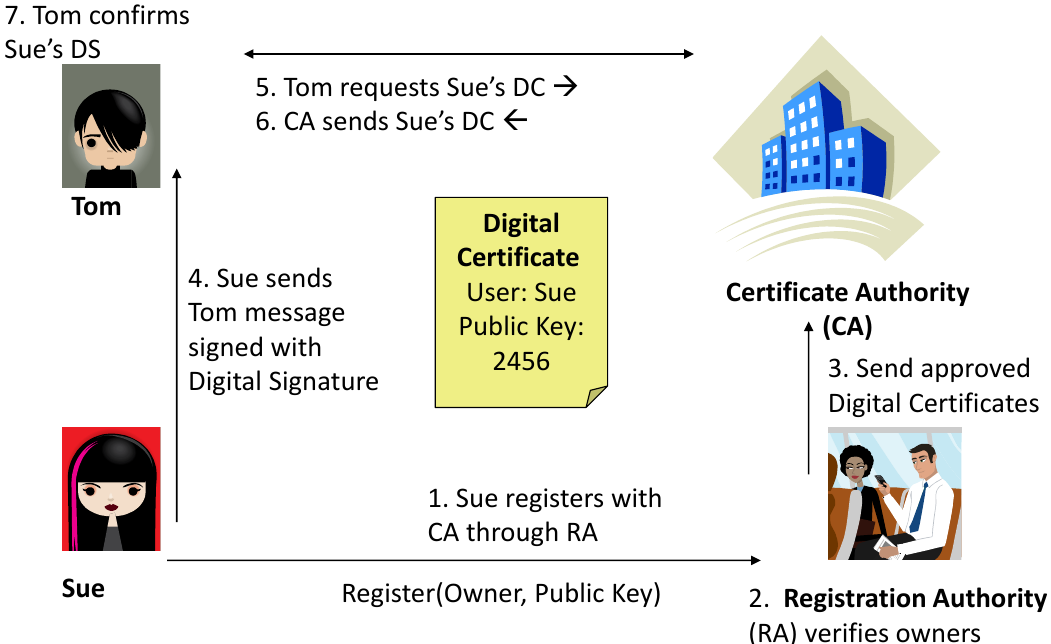
\includegraphics[scale=0.45]{publicKeyInfrastructure}
 \caption{Schema di funzionamento di una infrastruttura a chiave pubblica}
\end{figure}

Quindi in una CA sono presenti:
\begin{itemize}
\item I dati anagrafici;
\item L'algoritmo per eseguire la criptazione;
\item La propria chiave pubblica;
\item La firma della CA, fatta con la chiave privata.
\end{itemize}

I primi tre punti costituiscono $m$.

È anche presente un database pubblico con i certificati che sono stati 
revocati, questo per assicurare al venditore che prima di ogni transazione 
possa andare a verificare dalla CA che il certificato dell'acquirente è valido.

Esistono diverse CA.


\subsubsection{Network Access Server}

Un Network Access Server (NAS) presenta differenti caratteristiche. Un NAS gestisce
l'autenticazione degli utenti, compiendo l'\textit{access control} e
l'\textit{accounting} di essi. Una volta eseguito con successo un login,
vengono inviate al client le informazioni sull'utente (come ad esempio il suo
ID). Il problema dei NAS è che sono proni ad attacchi da parte di hackers, 
oltre a essere suscettibili di attacchi DOS.

Oggi questa modalità è stata soppiantata dalle VPN.

\subsection{Vulnerability Assessment}

\begin{itemize}
\item Scan servers, work stations e controllare i dispositivi per le
vulnerabilità (servizi open, patching, vulnerabilità delle configurazioni).
L'80\% degli attacchi avviene perché i sistemi non sono patchati. Alcune 
aziende prevedono nella policy che i sistemi devono essere patchati ogni $x$ 
mesi in modo da evitare vulnerabilità. Senza queste policy è difficile che si 
facciano;
\item Controlli e test per il corretto funzionamento
\begin{itemize}
 \item Aderenza alle policy e agli standard;
\end{itemize}
\item Penetration testing, molto utilizzato per le reti wireless, meno utile su
servizi web.
\end{itemize}

\section{Riassunto dei controlli di rete}

Riassumendo, i controlli di rete possono essere di tre tipologie:

\begin{enumerate}
 \item Tecniche di controllo di sicurezza della rete
 \begin{itemize}
  \item Criptazione;
  \item VPN;
  \item Hashing;
  \item Firme digitali;
  \item Configurazione host in modalità \textit{bastion};
  \item Certificato di autorità, infrastruttura a chiave pubblica;
 \end{itemize}

 \item Protezione dei \textit{device} nella rete
 \begin{itemize}
  \item Firewall;
  \item Proxy server;
  \item DMZ;
  \item Sistemi di rivelazione di intrusione;
  \item Sistemi di prevenzione di intrusione;
  \item NAS (\textit{network access server});
  \item \textit{Honeypot}, \textit{honeynet};
 \end{itemize}

 \item Protocolli di sicurezza
 \begin{itemize}
  \item SSL;
  \item SSH;
  \item S/MIME;
  \item Gestione dell'informazione sulla sicurezza: gestione dei log.
 \end{itemize}
\end{enumerate}



\section{Esercizi}

Gli esercizi riepilogativi su questa parte del corso si possono trovare in
\ref{EsNetRiep}.


\part{Risk Management}

\label{riskMng}

Quanto è importante investire nella sicurezza? La sicurezza è sempre più
``venduta'' e comunicata come il classico ROI\footnote{Ritorno d'investimento}.
C'è anche un altro fattore da tenere conto, la pubblicità: la cattiva
pubblicità è devastante per un'azienda e può danneggiare molto
facilmente la fiducia degli utenti. Si stima che ci sia un ritorno
dell'investimento del 5\%.

Non tutti i controlli vanno implementati, bisogna sapere a cosa mirare.
L'importante è convincere chi approva le scelte a spendere in sicurezza.



\chapter{Gestione del rischio}

La storia, il grado di maturità, la cultura, la società e la tolleranza
influiscono sul rischio. Esistono anche dei fattori esterni, che sono le
\textit{regulation}, ovvero le normative e le leggi. Il fattore esterno è la
motivazione più forte oggigiorno, in quanto son previsti anche sanzioni di tipo
penale.

L'altro fattore esterno è la \textit{industry}, ossia confrontarsi con i propri
competitor.

\textbf{Risk tolerance:} come il management vive la percezione del rischio
(quanto rischio è disposto ad accettare).

\section{Risk Management Process}
La gestione del rischio si suddivide nei seguenti in passi:
\begin{enumerate}
\item Individuazione dei limiti e dei contesti;
\item Valutazione (assessment) del rischio:
\begin{itemize}
  \item Identificazione (Asset: materiali, non 
  materiali\footnote{es. reputazione});
  \item Analisi;
  \item Valutazione.
\end{itemize}
\item Trattamento del rischio:
\begin{itemize}
  \item Evitare;
  \item Ridurre;
  \item Trasferire;
  \item Mantenere.
\end{itemize}
\item Accettare il rischio residuo.
\end{enumerate}

\begin{figure}[H]
 \centering
 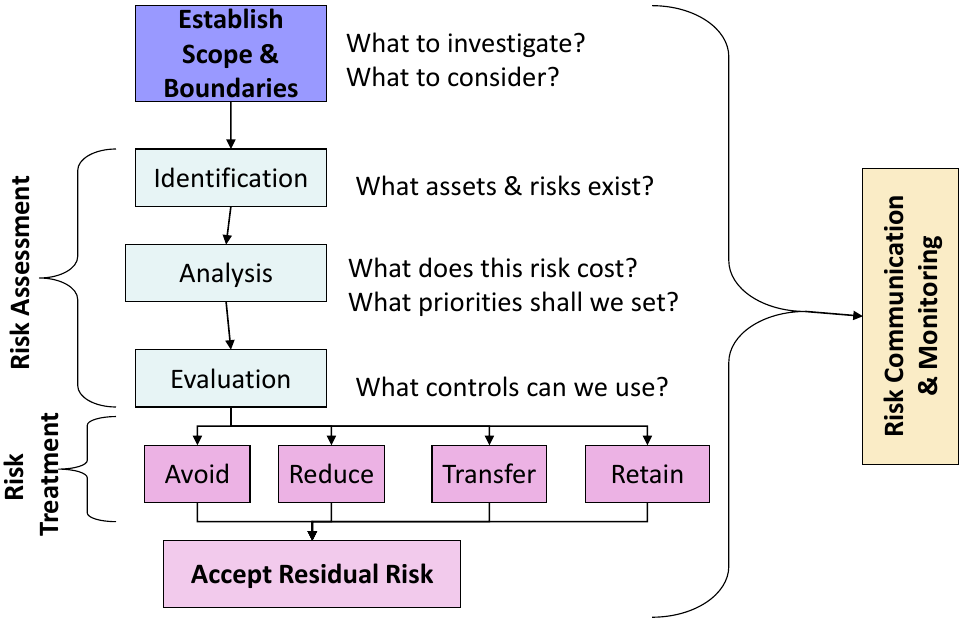
\includegraphics[scale=0.5]{riskManagementProcess}
 \caption{Schema del processo di gestione del rischio}
\end{figure}

Il rischio si può ridurre, mantenere, trasferire, evitare. Alla fine rimane il
rischio residuo, dove bisogna decidere se questo rischio è sopportabile o meno,
o se ci sono miglioramenti che sono possibili da intraprendere. In caso sia
possibile eseguire un'ulteriore riduzione del rischio si reitera il processo.

Una volta che il lavoro è stato fatto, dev'essere comunicato alle varie
persone incaricate. Il monitoraggio è una parte fondamentale del PDCA, che
permette un miglioramento continuo.

\section{Risk Appetite}

Come una persona si pone nel confronto del rischio (es. aprire mail che dentro
hanno spam, dare i dati della carta di credito).

È sempre meglio eseguire una valutazione piuttosto che scegliere
``a scatola chiusa''.


\section{Processo di Risk Management}

Si parte con il \textit{Risk appetite} per identificare il rischio, per poi
muoversi verso la creazione di un piano della gestione del rischio, che deve 
essere implementato. Siccome i rischi si evolvono e continuano a
cambiare, è importate eseguire un \textit{monitoring} continuo del rischio. 
Bisogna tenere in considerazione il fatto che i controlli potrebbero
introdurre delle nuove vulnerabilità.

Di conseguenza, il processo dev'essere iterativo in quanto l'ambiente è
dinamico.


\subsection{Risk Assessment}

È formato da 5 step:
\begin{enumerate}
 \item Assegnazione dei valori agli \textit{assets}. Solitamente è presente
il problema dell'identificazione dei \textit{Crown Jewels} (gioiello della
corona) ovvero gli \textit{assets} che valgono buona parte del totale (es.
brevetto particolare che è il core business).
 \item Determinazione della perdita dovuta e vulnerabilità nel sistema
 \item Stima della possibilità di un attacco portato a termine con successo
(ogni quanto potrebbe accadere?)
 \item Calcolare l'eventuale perdita. Son sempre da tenere a mente le seguenti
formule:
 \begin{itemize}
 	\item $Perdita\ =\ Downtime\ +\ Recovery\ +\ Liability\ +\ Replacement$
 	\item $Esposizione\ al\ rischio\ =\ Vulnerability\ \cdot\ Loss$
 \end{itemize}
 \item Gestione del rischio
\end{enumerate}

Ogni punto verrà spiegato meglio nei successivi paragrafi.


\subsubsection{Assegnazione dei valori agli assets}

Quando eseguo \textit{risk assessment} non è possibile contare tutti gli 
oggetti all'interno di un'azienda. È quindi importante individuare solamente 
tutto quello che veramente conta per la società.

\paragraph*{In pratica}

Per agire bisogna valutare l'ultimo \textit{risk assessment} che è stato
effettuato e bisogna vedere se ci sono state aggiunte o rimozioni.

Una volta identificati gli \textit{assets} più importanti, è necessario
calcolarne il valore, cosa che spesso non risulta essere semplice\footnote{Ad
esempio il costo di un determinato Software}. Bisogna inoltre calcolare il 
costo di una eventuale \textit{recovery}.



\subsubsection{Determinare la perdita causata dalle vulnerabilità e dalle
minacce}

Bisogna assegnare un valore a questi oggetti, soprattutto se immateriali. 
Spesso per i beni immateriali (come la reputazione) si riesce a valutare il 
valore effettivo solamente dopo che la perdita è avvenuta.

Le perdite vengono calcolare su confidenzialità, integrità e disponibilità.

\paragraph*{In pratica}

Esistono i costi tangibili e intangibili. Sono presenti anche il costo del
rimpiazzo e quelli legate alle perdite.
Il costo dal punto di vista intangibile è di tipo qualitativo, e non
quantitativo.


\subsubsection{Stimare la probabilità di exploit}

Si valuta qual è la probabilità che un evento malevolo mi colpisca tramite
indagini, interviste e casi simili già accaduti.

\paragraph*{In pratica}

L'esperienza passata, la definizione degli standard internazionali, i consigli
di specialisti ed esperti nel settore, ricerche di mercato e esperimenti
tramite prototipi sono diversi modi da cui è possibile attingere
informazione per capire quanto si è esposti ad un possibile \textit{exploit}.



\subsubsection{Calcolare la perdita attesa}

La perdita è composta dal \textit{downtime}, \textit{recovery},
\textit{liability} e il rimpiazzo del prodotto. Il costo del rimpiazzo spesso è
minore di tutto quello che ci sta prima: ovvero tutti i costi che vengono a
crearsi a causa della disfunzione creata.

\paragraph*{In pratica}

Per calcolare la perdita attesa esistono tre tipologie di calcolo: la stima
\textbf{qualitativa}, quella \textbf{quantitativa} e quella
\textbf{semiquantitativa}.

\begin{itemize}
\item Qualitativa: corretta perché riuscite a prioritizzare i rischi, quindi
capire cosa è più importante di cosa;
\item Quantitativa: la più corretta perché in qualche modo riporta in una scala
assoluta (es. soldi). Il problema è definire una valutazione corretta;
\item Semiquantitativa: mix tra le prime due.
\end{itemize}

\subparagraph*{Analisi qualitativa}

L'analisi qualitativa è usata:
\begin{itemize}
\item Come analisi preliminare per i rischi;
\item Con asset non tangibili come la reputazione e l'immagine;
\item Quando non sono presenti sufficienti informazioni per eseguire 
un'analisi quantitativa.
\end{itemize}

\subparagraph*{Analisi quantitativa}

\begin{itemize}
\item Single Loss Expectancy (\textbf{SLE}): il costo per l'organizzazione se 
una minaccia si verifica:
$$
\text{SLE} = \text{ASSET VALUE (\textbf{AV})} \cdot \text{ Exposure Factor 
(\textbf{EF})};
$$
\item Annualized Rate of Occurrence (\textbf{ARO}): quanto frequentemente o 
quanto probabile è che l'evento si verifichi in un anno?
\item Annual Loss Expectancy (\textbf{ALE}): la perdita attesa annuale è dato 
da
$$
\text{ALE} = \text{SLE} \cdot \text{ARO}.
$$
\end{itemize}

Quanto si perde del bene se l'evento capita?

Sull'anno questo evento quanto mi costa? L'evento negativo ha sicuramente un
certo costo, ma che impatto ha all'anno? Se per esempio un'alluvione avviene
ogni 30 anni, allora il suo costo è $1/30$ all'anno. Quindi ogni anno l'azienda
deve risparmiare un certo valore per far fronte alla perdita futura.

\subsubparagraph*{Esempio}

Quantitativamente:
\begin{itemize}
\item Il costo di un incidente HIPAA con protezioni insufficienti:
\begin{itemize}
 \item SLE = 50k + (1 anno in prigione) \$ 100k = \$150k;
 \item Più perdite in termine di reputazione.
\end{itemize}
\item Stima del tempo = 10 anni o meno = 0.1;
\item Stime di perdita annuale (ALE): \$150k $\cdot$ 0.1 = \$15k.
\end{itemize}


\begin{figure}[H]
 \centering
 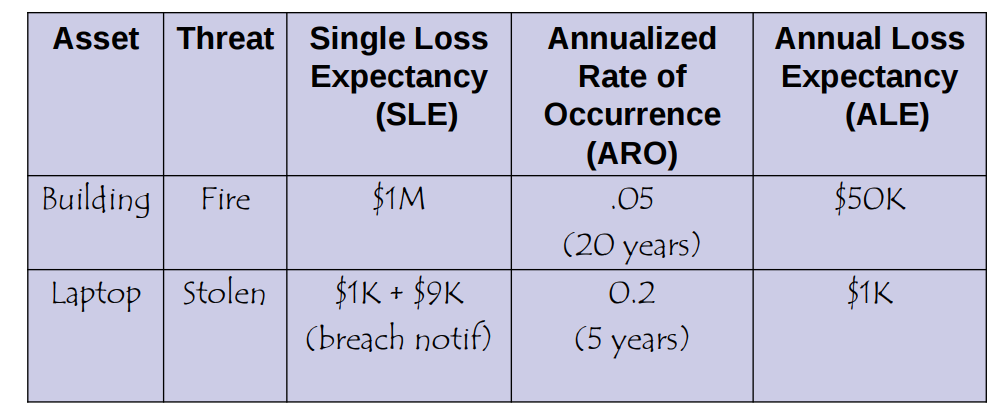
\includegraphics[scale=0.32]{quantitative_risk}
 \caption{Esempio per chiarire SLE, ARO e ALE.}
\end{figure}

Le \textit{Security breach notification laws} sono leggi che impongono ad 
entità che sono state soggette a furti di dati di notificarlo ai clienti e di 
prendere contromisure per cercare di rimediare alle possibili conseguenze. 
Esiste una direttiva europea a riguardo.


\paragraph*{Tipologie di Minacce}
Nella Figura \ref{fig:threat:types} vengono riportate le diverse 
tipologie di minacce.
\begin{figure}[H]
 \centering
 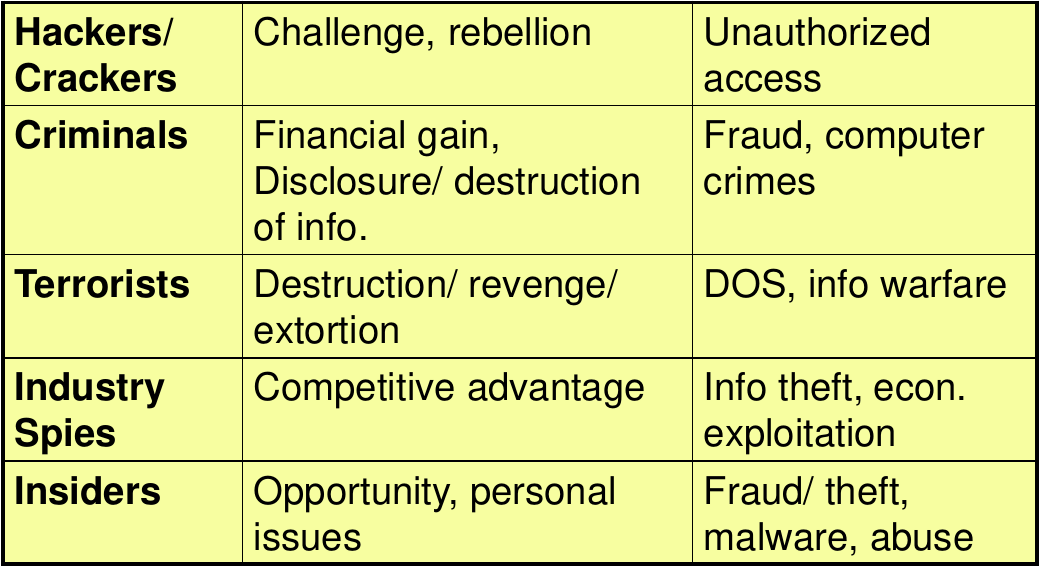
\includegraphics[scale=0.365]{threatAgentTypes}
 \caption[Tabella delle differenti tipologie di minacce]{Tabella delle 
 differenti tipologie di minacce: nella prima colonna sono riportati
 i tipi di agenti, nella seconda le motivazioni e nell'ultima colonna
 le conseguenze di queste minacce.}
 \label{fig:threat:types}
\end{figure}


\paragraph*{Come difendersi}

Per difendersi le grandi società di software eseguono delle settimane di
allenamento per i programmatori, definite anche come \textit{security coding}.



\subsubsection{Trattamento dei rischi}

Si eseguono delle \textit{survey} e si controllano i rischi esistenti. Se non
dovesse essere abbastanza, vengono aggiunti nuovi controlli.

Con il trattamento del rischio viene deciso se evitare, trasferire, mantenere,
mitigare o pianificare il rischio.

\begin{itemize}
\item \textbf{Accettazione} del rischio: è importante prendere delle decisioni 
riguardo all'accettazione del rischio;
\item \textbf{Evitare} il rischio: bloccare i comportamenti che causano 
esposizione al rischio;
\item \textbf{Mitigazione} del rischio: implementare dei controlli per 
minimizzare le vulnerabilità sotto un livello accettabile;
\item \textbf{Trasferimento} del rischio: qualcun altro assume il rischio per 
l'azienda (es. ricorrere ad un'assicurazione);
\item \textbf{Pianificazione} del rischio: implementare una serie di 
contromisure. Che controlli dovrebbero essere messe in piedi?
\end{itemize}

\begin{figure}[H]
 \centering
 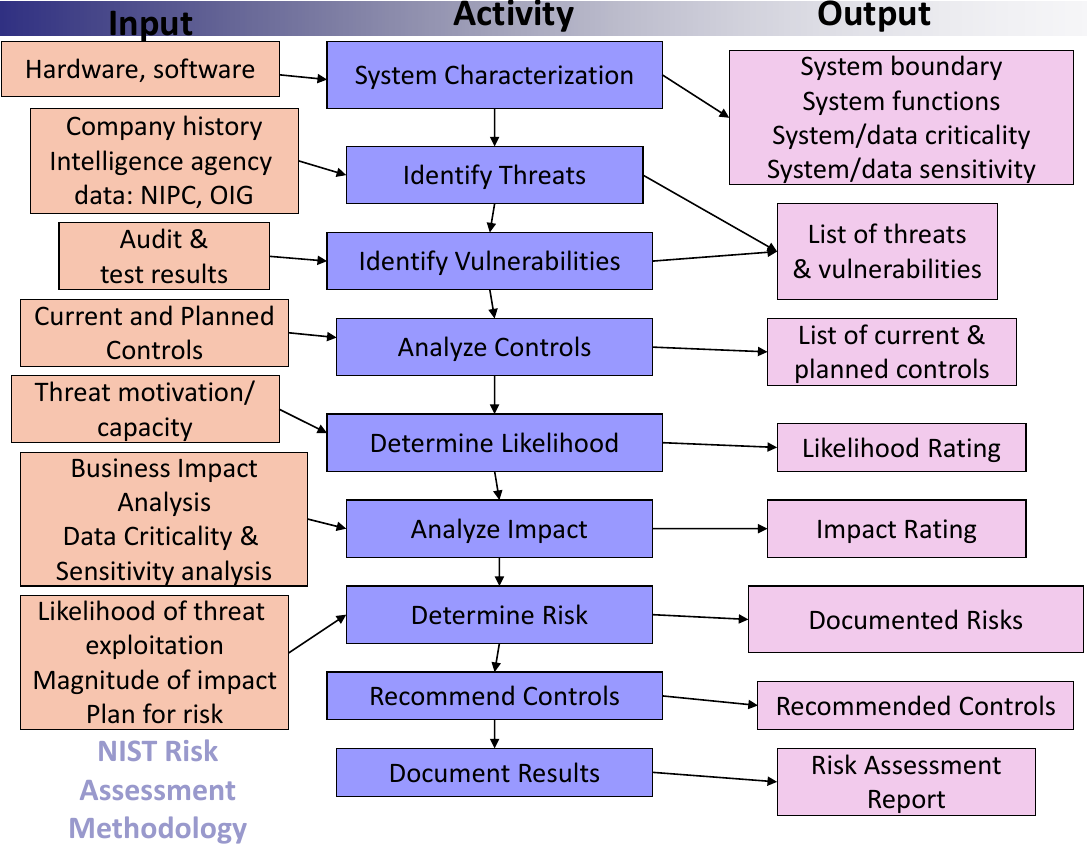
\includegraphics[scale=0.5]{treatRisk}
 \caption{Schema di come dovrebbe essere trattato il rischio}
\end{figure}



Ad un certo punto potrebbe non essere più possibile eliminare il rischio. Il
rischio che rimane viene detto \textbf{rischio residuo} e questo rischio viene
accettato.

La \textit{sensitivity analysis} indica quanto l'azienda è ``sensibile'' a 
certi avvenimenti.

Il \textit{risk assessment} va fatto solo su una parte dell'azienda, non su
tutte.

\paragraph*{In pratica}

Per alcuni eventi ci si basa sull'esperienza passata (es. eventi atmosferici).
Per eventi per cui non è possibile basarsi sulle esperienze precedenti ci si
basa su delle \textit{guidelines}.

\paragraph*{Fonti di perdite}

Archetipi:
\begin{itemize}
\item Utente malintenzionato (o malizioso): vuole causare un danno all'azienda;
\item Utente non intenzionale: causa un danno all'azienda ma senza volerlo;
\item Utente che piega le regole: in qualche modo è a metà tra i due profili
precedenti. Le sue azioni sono intenzionali, ma non maliziose.
\end{itemize}

Il 51\% pensa sia accettabile prendere dati dell'azienda perché pensano che sia
normale farlo in assenza di \textit{policy}. Molti dati vengono passati
nell'azienda tramite \textit{Dropbox} o su \textit{Gmail}. Altri eseguono
download illegali sul computer aziendale. Essenzialmente, c'è poco controllo 
sui dati, dimostrando come un utente può avere un atteggiamento malizioso senza
troppi problemi.
